%%%%%%%%%%%%%%%%%%%%%%%%%%%%%%%%%%%%%%%%%%%%%%%%%%%%%%%%%%%%%%%%%%%%%%%%%%%%
\documentclass[a4j]{jarticle}

\usepackage{jsaisig}
% \usepackage{graphicx}
\usepackage[dvipdfmx]{graphicx}
\usepackage{subfigure}
\usepackage{multirow}
% \usepackage{}

%%%%%%%%%%%%%%%%%%%%%%%%%%%%%%%%%%%%%%%%%%%%%%%%%%%%%%%%%%%%%%%%%%%%%%%%%%%

\begin{document}

% 和文タイトル
\title{Find My Matesに向けた解法の提案と実機での性能評価}

% 英文タイトル
\etitle{Solution of Find My Mates and evaluation on Domestic Standard Robot}

% 著者名:
%	・各著者を\quad(全角空白)区切りで列挙
% 	・著者名の直後に\afil{所属番号}を追加→所属番号を上付で出力(\textsuperscript{所属番号}と同じ)
% 	 複数機関へ所属している場合は番号をカンマ区切りで列挙(下記著者2参照)
%  ・Corresponding Authorについては所属の後に\thanksを続け,連絡先を記入
%	・英文著者はカンマ区切りで列挙

\author{矢野 優雅\afil{1}%
	\thanks{連絡先:九州工業大学大学院生命体工学研究科人間知能システム工学専攻 \newline%
		      〒808-0135 福岡県北九州市若松区ひびきの2-4 \newline%
		      E-mail: yano.yuuga158@mail.kyutech.jp}\quad%
	福田 有輝也\afil{1}
	小野 智寛\afil{1}
	田向 権\afil{1,2}\\
	Yuga Yano\afil{1}, Yukiya Fukuda\afil{1}, Tomohiro Ono\afil{1}, and Hakaru Tamukoh\afil{1,2}}

% 所属
\affiliation{%
	\afil{1} 九州工業大学大学院生命体工学研究科\\
	\afil{1} Graduate School of Life Science and Systems Engineering, Kyushu Institute of Technology, Japan\\
	\afil{2} ニューロモルフィックAIハードウェア研究センター\\
	\afil{2} Research Center for Neuromorphic AI Hardware, Kyushu Institute of Technology, Japan}

\abstract{
% Abstract (English) comes here.......................................................
ホームサービスロボットの技術発展を目的として,RoboCup@Homeという競技会が開催されている.
RoboCup@Homeでは,実際の家庭環境を模したフィールドを用いてタスクを行うことで,より現実に近い環境でロボットの性能を評価することができる.
本研究では,RoboCup@Homeのタスクの一つであるFind My Matesに向けて,満点を取得するための手法を提案する.
また,提案した手法をロボットに実装し,2022年7月にバンコクで行われたRoboCup@Homeにて現地実験を行った.
現地実験では満点を取得し,提案手法の有効性を示した.
}

\maketitle
\thispagestyle{empty}

%%%%%%%%%%%%%%%%%%%%%%%%%%%%%%%%%%%%%%

\section{序論}
% テストと競技表記ゆれが起きそうなので,早いうちに確定させる
\subsection{RoboCup@Home}
RoboCup@Homeは,ホームサービスロボットの技術発展を目的に開催されている競技会である.
本競技会では,人間とロボットの協調を目標の一つに掲げており,
音声認識や物体認識,ナビゲーションといった動的環境におけるテストが行われている.
そのため,より現実環境を想定した性能評価をすることができ,非常に注目を集めているリーグとなっている.
% The RoboCup@Home league aims to develop service and assistive robot technology with high relevance for future personal domestic applications. It is the largest international annual competition for autonomous service robots and is part of the RoboCup initiative. A set of benchmark tests is used to evaluate the robots’ abilities and performance in a realistic non-standardized home environment setting. Focus lies on the following domains but is not limited to: Human-Robot-Interaction and Cooperation, Navigation and Mapping in dynamic environments, Computer Vision and Object Recognition under natural light conditions, Object Manipulation, Adaptive Behaviors, Behavior Integration, Ambient Intelligence, Standardization and System Integration. It is colocated with the RoboCup symposium.
RoboCup@Homeには,Open Platform,Domestic Standard Platform(DSPL),Social Standard Platformという3つのリーグがある.
私たちの参加しているDSPLでは,トヨタ社が開発したHuman Support Robot(HSR)\cite{hsr_paper}を標準機に採用しテストを行っている.
図\ref{overview_hsr}に,HSRの外観と搭載されているデバイスを示す.
\begin{figure}[ht]
  \centering
  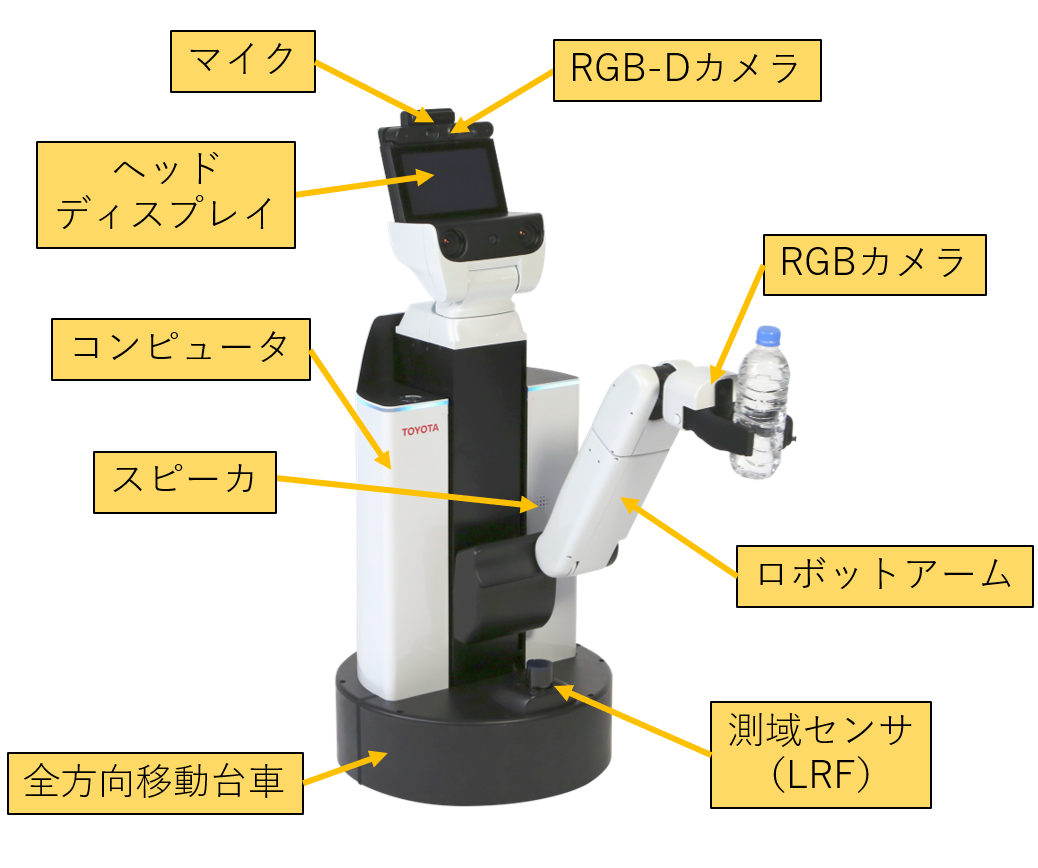
\includegraphics[width=6cm]{images/hsr/hsr_explain_ja.png}
  \caption{トヨタ社が開発したHSR}
  \label{overview_hsr}
\end{figure}
HSRは移動台車やアームに加えて,RGB-Dカメラやマイクが搭載されており,認識を通して多様なヒューマンインタラクションを行うことができる.

本研究では,ヒューマンインタラクションの性能をはかるFind My Matesというテストに向けて,その解法を提案するとともに,HSRへの実機実装を行いRoboCup@Homeでの性能評価を行う.

% 2ページ目の先頭に持ってくるため
\begin{figure*}[ht]
  \centering
  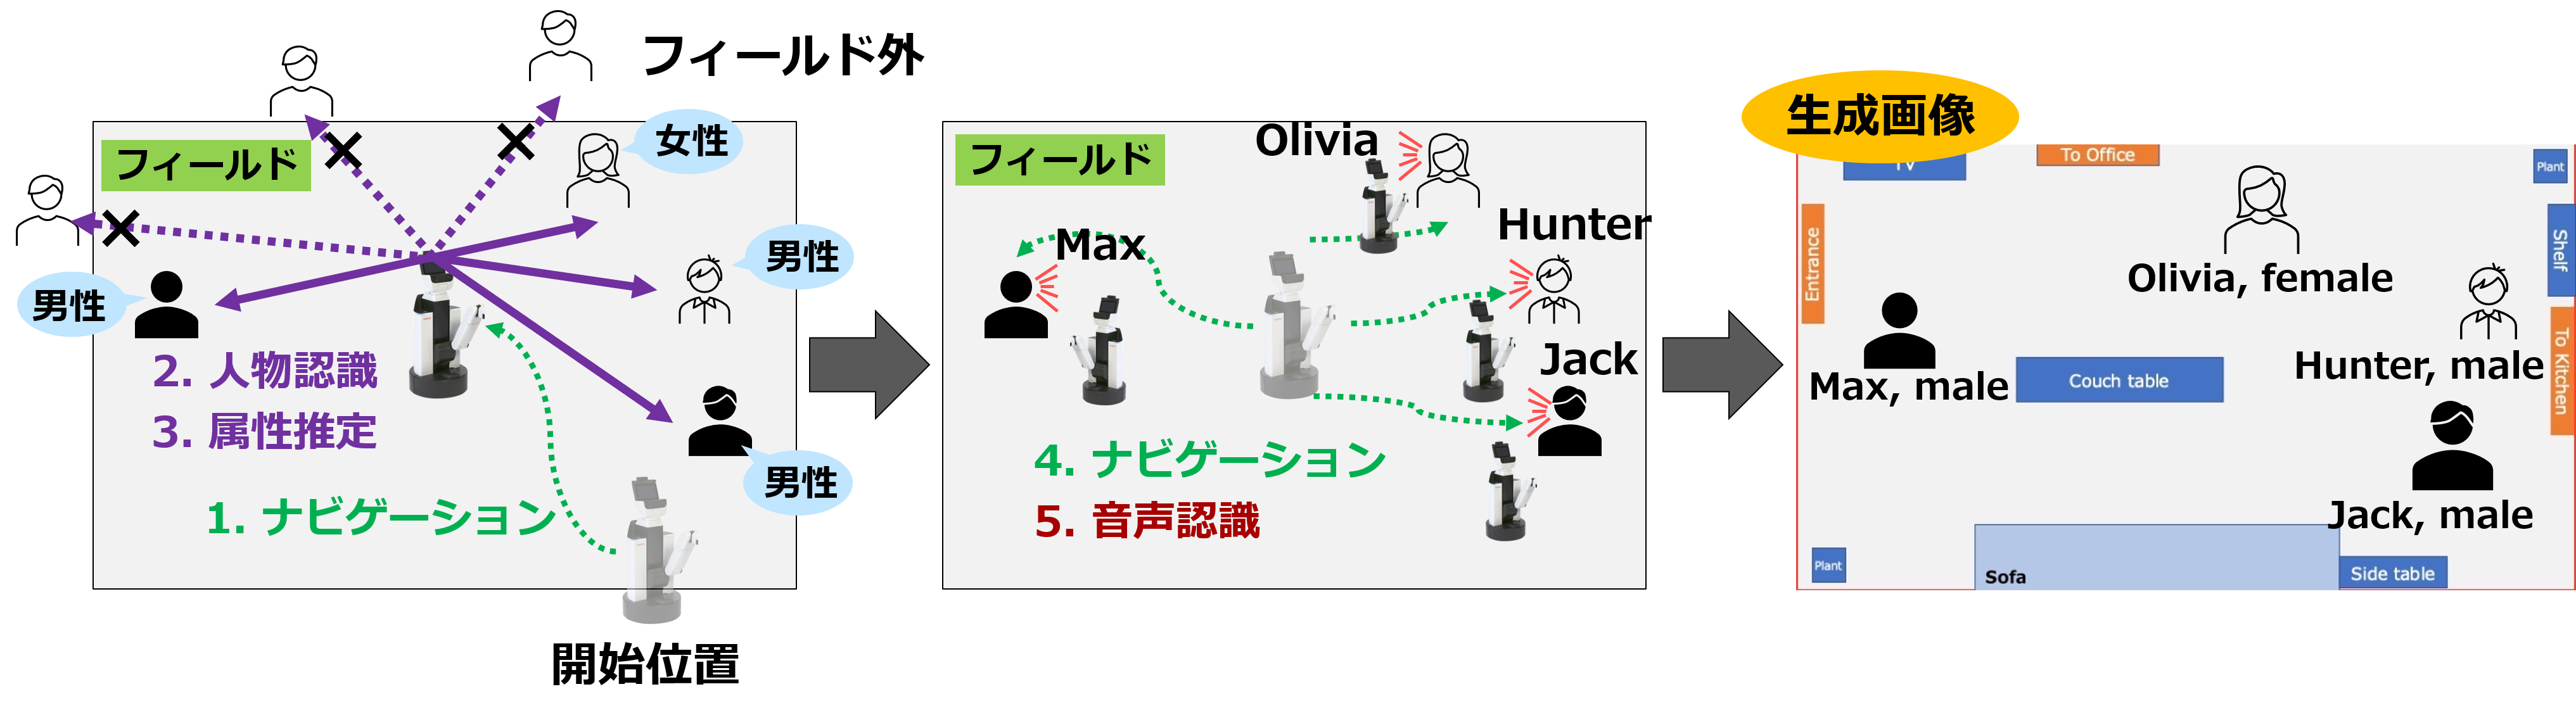
\includegraphics[width=16cm]{images/FMM/solution_overview_yoko_yy2.png}
  \caption{FMMの解法}
  \label{solution_overview}
\end{figure*}

\subsection{Find My Mates}
本章では,RoboCup@Homeで行われるFind My Mates(FMM)というタスクについて述べる.
FMMでは,4人のゲストが1人のホストを訪れたという状況を想定している.
% しかし,ホストはゲストの名前のみを知っているがその他の情報は何も知らない.
FMMは,1人のホストの家に訪れた4人のゲストをロボットが探し,その場所,名前に加えて人物の特徴をホストに報告するというタスクである.
そのため,人物を3次元的に認識する技術と,それぞれのゲストの特徴を抽出する属性推定の技術が必要になる.
更に,ロボットは事前にゲストの名前を知らされていないため,音声認識を通してゲストの名前を知る必要がある.

\section{関連研究}


\section{提案手法}
本章では,FMMで満点を取得する解法と,HSRに実装した機能について述べる.
% FMMでは部屋に移動した後,4人のゲストを見つける必要がある.

\subsection{FMMに向けた解法}
私達はFMMで満点を取得するために,次のような解法を提案する.
提案する手法の概要を図\ref{solution_overview}に示す.
初めに,ロボットを部屋の中央までナビゲーションを行い,部屋全体を見渡しながら人物認識を行う.
ここで,Depth画像も用いることで,認識した人がmap上のどこにいるのかを算出する.
% 次に,認識した人がエリア内のどこにいるかの判定を行う.これには,大きく2つの理由がある.
% 1つは,ロケーション報告に用いるためであり,
% もう1つは,フィールド周囲の観客の誤認識を防ぐためである.
算出した人物の位置情報を基に,各ゲストの正面までナビゲーションを行い,名前を聞く.
更に,属性推定の手法を用いて,ゲストの性別を推定する.

最後に,取得したすべての情報(人物の画像,位置,名前,性別)を集約した1枚の画像を作成し,
ヘッドディスプレイに表示することでホストに伝える.

\subsection{音声認識}
近年ではスマートフォンなどの普及により,Siriなどのクラウドを用いた音声認識の精度が非常に高くなっている.
しかし,RoboCup@Homeでは会場のネットワークが不安定である場合が想定され,安定したクラウド上での音声認識が困難である.
また,ネットワークの課題は一般の家庭環境においても想定されるものであり,オフラインでの音声認識技術を利用することは非常に有効である.
そこで本研究では,vosk\cite{vosk_hp}と呼ばれるオフラインの手法を用いて音声認識を行う.

本研究では,音声認識を図のように実装している.
HSRのヘッド部に搭載されているマイクを用いて,一定時間録音する.
次に,録音した音声をROSを介してPCに送信する.
ここで,ROSには音声ファイルをそのまま送信できるメッセージ型がないため,音声ファイルをnumpyの配列に読み直して送信を行う.
PC側では,受信したnumpyの配列から音声ファイルを再構築し,音声認識を行う.
% 音声ファイルをROSで通信したことも書く.
% 音声認識を一定時間で行っていることも書く
% 音声認識の結果の評価があっても面白い
% 一回でも認識できなかったら,そのタスク中は音声認識をあきらめる事もかいておくべき

\subsubsection{辞書設定}
RoboCup@Homeでは,タスクに登場する人物は本名を使用するのではなく,
事前に公開している名前リストから毎回ランダムに決定され名前を割り当てられる.
この名前リストには,男性用と女性の用の名前が約10個ずつ用意されている.
ただし,名前だけで性別の区別ができないようにするために,男性と女性で共通している名前も存在する.
今回は,このvoskを使用する際に名前リストをもとにした辞書を作成し,名前の音声認識精度向上を行う.
% ここ定量的な表現に直す
辞書を設定していない場合では,名前を話してもまったく違う単語として認識されることがほとんどであったが,
辞書設定をすることで認識率は飛躍的に向上した.

\subsection{ノイズ除去}
RoboCup@Homeは実際の家庭環境を模したフィールドで行われるが,実際の家庭環境と異なる点もある.
その一つが,周囲のノイズが大きいことである.
RoboCup@Homeの他にも,サッカーリーグやレスキューリーグが同時に行われているため,実際の家庭環境では起きないような大きなノイズが発生する.
本研究では,音声認識の精度を高めるために,ノイズ除去\cite{sainburg2020finding}を音声認識の前段に組み込み,精度を高めている.
% これに定量的な実験結果を載せてもいいと思う

\subsection{音声認識の性能評価}
RoboCup@Homeで使用される名前は,アメリカで一般的に用いられる名前からランダムに決定される.
そこで,本研究で作成した音声認識の性能を評価するため,
アメリカで一般的に使用されている名前から男女それぞれ名前を11個選出し,認識精度を検証した.
検証はノイズの大きな環境で行い,話者とノイズの環境を変化させながらそれぞれ4度ずつ読み上げて検証を行った.

表\ref{voice_recognition_result}に,ノイズ除去を行った場合と辞書指定を行った場合における認識結果を示す.
\begin{table}[]
	\centering
	\caption{音声認識の精度}
	\begin{tabular}{|c|c|c|}
	\hline
	辞書指定                & ノイズ除去 & 認識精度(\%)          \\ \hline
	\multirow{2}{*}{なし} & なし    & 13.6          \\ \cline{2-3}
	                    & あり    & 10.2          \\ \hline
	\multirow{2}{*}{あり} & なし    & 69.3          \\ \cline{2-3}
	                    & あり    & \textbf{71.6} \\ \hline
	\end{tabular}
	\label{voice_recognition_result}
\end{table}

\subsection{人物認識}
本研究では人物認識の手法にLightweight Human Pose Estimation\cite{light-openpose}を用いた.
本手法は処理が非常に軽量であり,CPUでも高速に動作できる手法である.
今回使用したPCでは,x fpsで動作しており,HSRのカメラ周期と同等な速度である為,
リアルタイム動作を実現できていると言える.
本研究では,人物を3次元的に認識する必要があるため,RGB画像から人物認識を行った後,
認識位置のDepth画像を参照することで,3次元的な位置を推定する.
図\ref{human_estimation_explain}に,人物の3次元的な位置推定を行った結果を示す.
\begin{figure}[ht]
  \centering
  \subfigure[RGB画像での認識結果]{
  	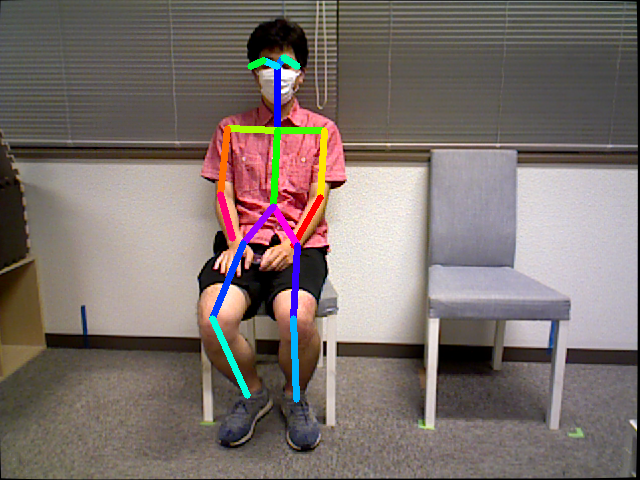
\includegraphics[height=3cm]{images/human_recognition/image.png}
	\label{human_estimation_image}
	% \caption{RGB画像での認識結果}
  }
  % \subfigure[Depth画像と合わせた3次元の位置推定]{
  \subfigure[3次元の位置推定]{
  	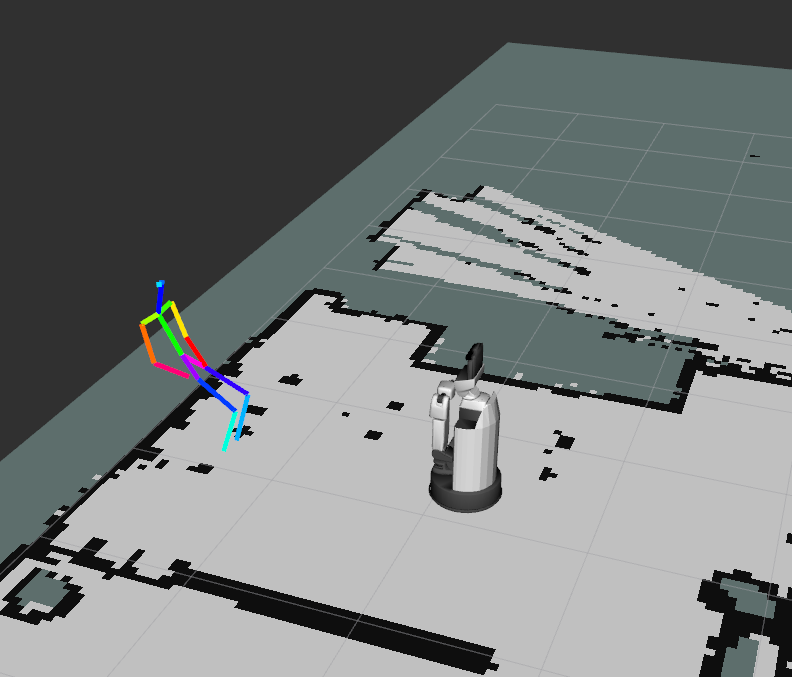
\includegraphics[height=3cm]{images/human_recognition/ss_4_trim.png}
	\label{human_estimation_pc}
	% \caption{Depth画像と合わせた3次元の位置推定}
  }
  \caption{人物位置推定アルゴリズム}
  \label{human_estimation_explain}
\end{figure}

\subsection{ロケーション報告}
FMMでは,認識した人物をホストに伝える必要があるが,この際に考慮すべきこととして,
認識した人が本当に部屋の中にいる人なのか,部屋の中のどこにいるのかを識別する必要がある.
そこで本研究では,事前に作成しているマップに対してjsonファイルを用いて意味づけを行い,フィールド内判定を行う.
またRoboCup@Homeでは,事前に部屋の形が公開されるため部屋の中のどこに椅子があるのかという意味づけも行う.
人物のフィールド内判定と,位置推定の結果を図\ref{human_where_map}に示す.
\begin{figure}[ht]
  \centering
  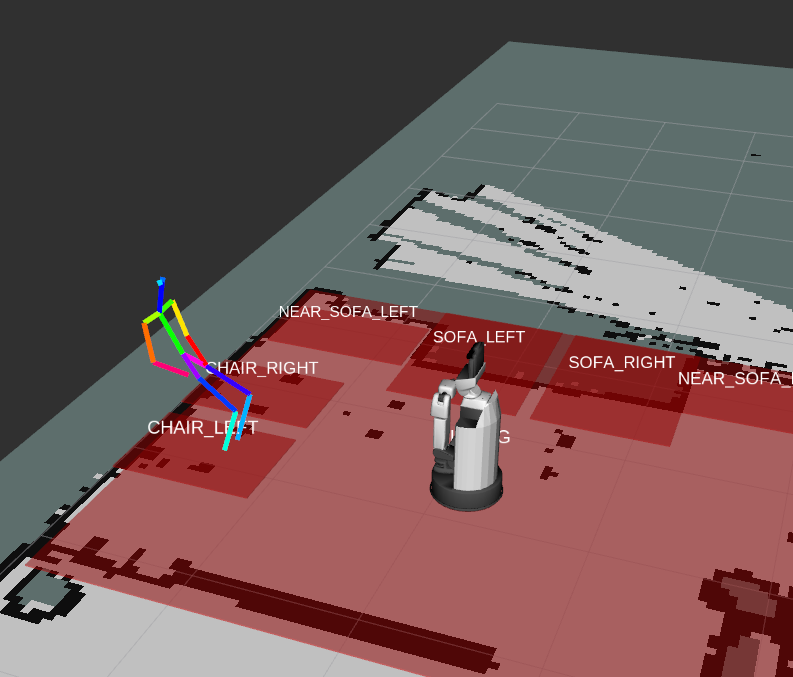
\includegraphics[width=6cm]{images/human_recognition/ss_5_trim.png}
  \caption{図\ref{human_estimation_explain}で認識した結果にエリア判定を付加した結果}
  \label{human_where_map}
\end{figure}
この場合では,ゲストはフィールド内の左側の椅子に座っており,それを正しく判定できている.

%%%%%%%%%%%%%%%%%%%%%%%%%%%%%%%%%%%%%%

\section{現地実験概要}
提案手法をHSRに実装し,2022年7月にバンコクで行われたRoboCup@Homeで性能評価を行った.
図\ref{robocup_field}に,実際に使用されたフィールドを示す.
\begin{figure}[ht]
  \centering
  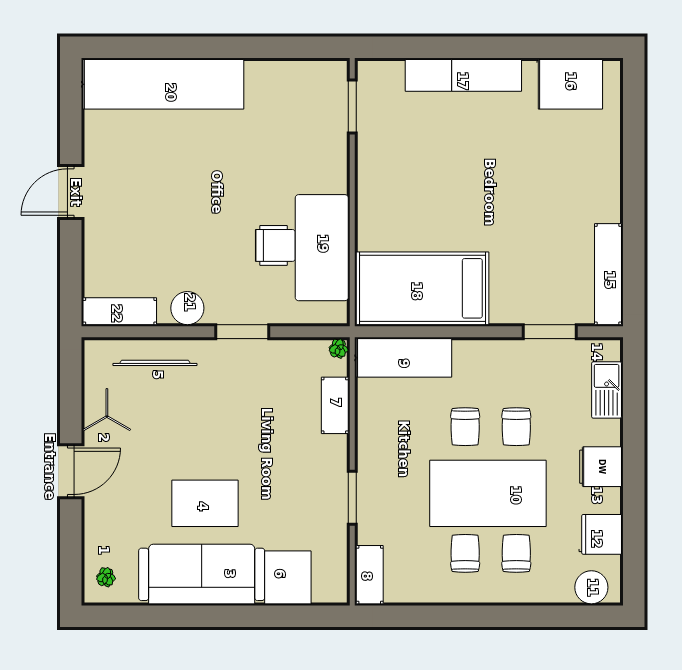
\includegraphics[width=6cm]{images/robocup/arenaBangkok_rotate.png}
  \caption{バンコクで開催されたRoboCup@Home2022で使用されたフィールド}
  \label{robocup_field}
\end{figure}
4つのルームがある中で,FMMはリビングルームにて実施された.
現地の実際の写真を図\ref{onsite_overview_1}に示す.
\begin{figure}[ht]
  \centering
  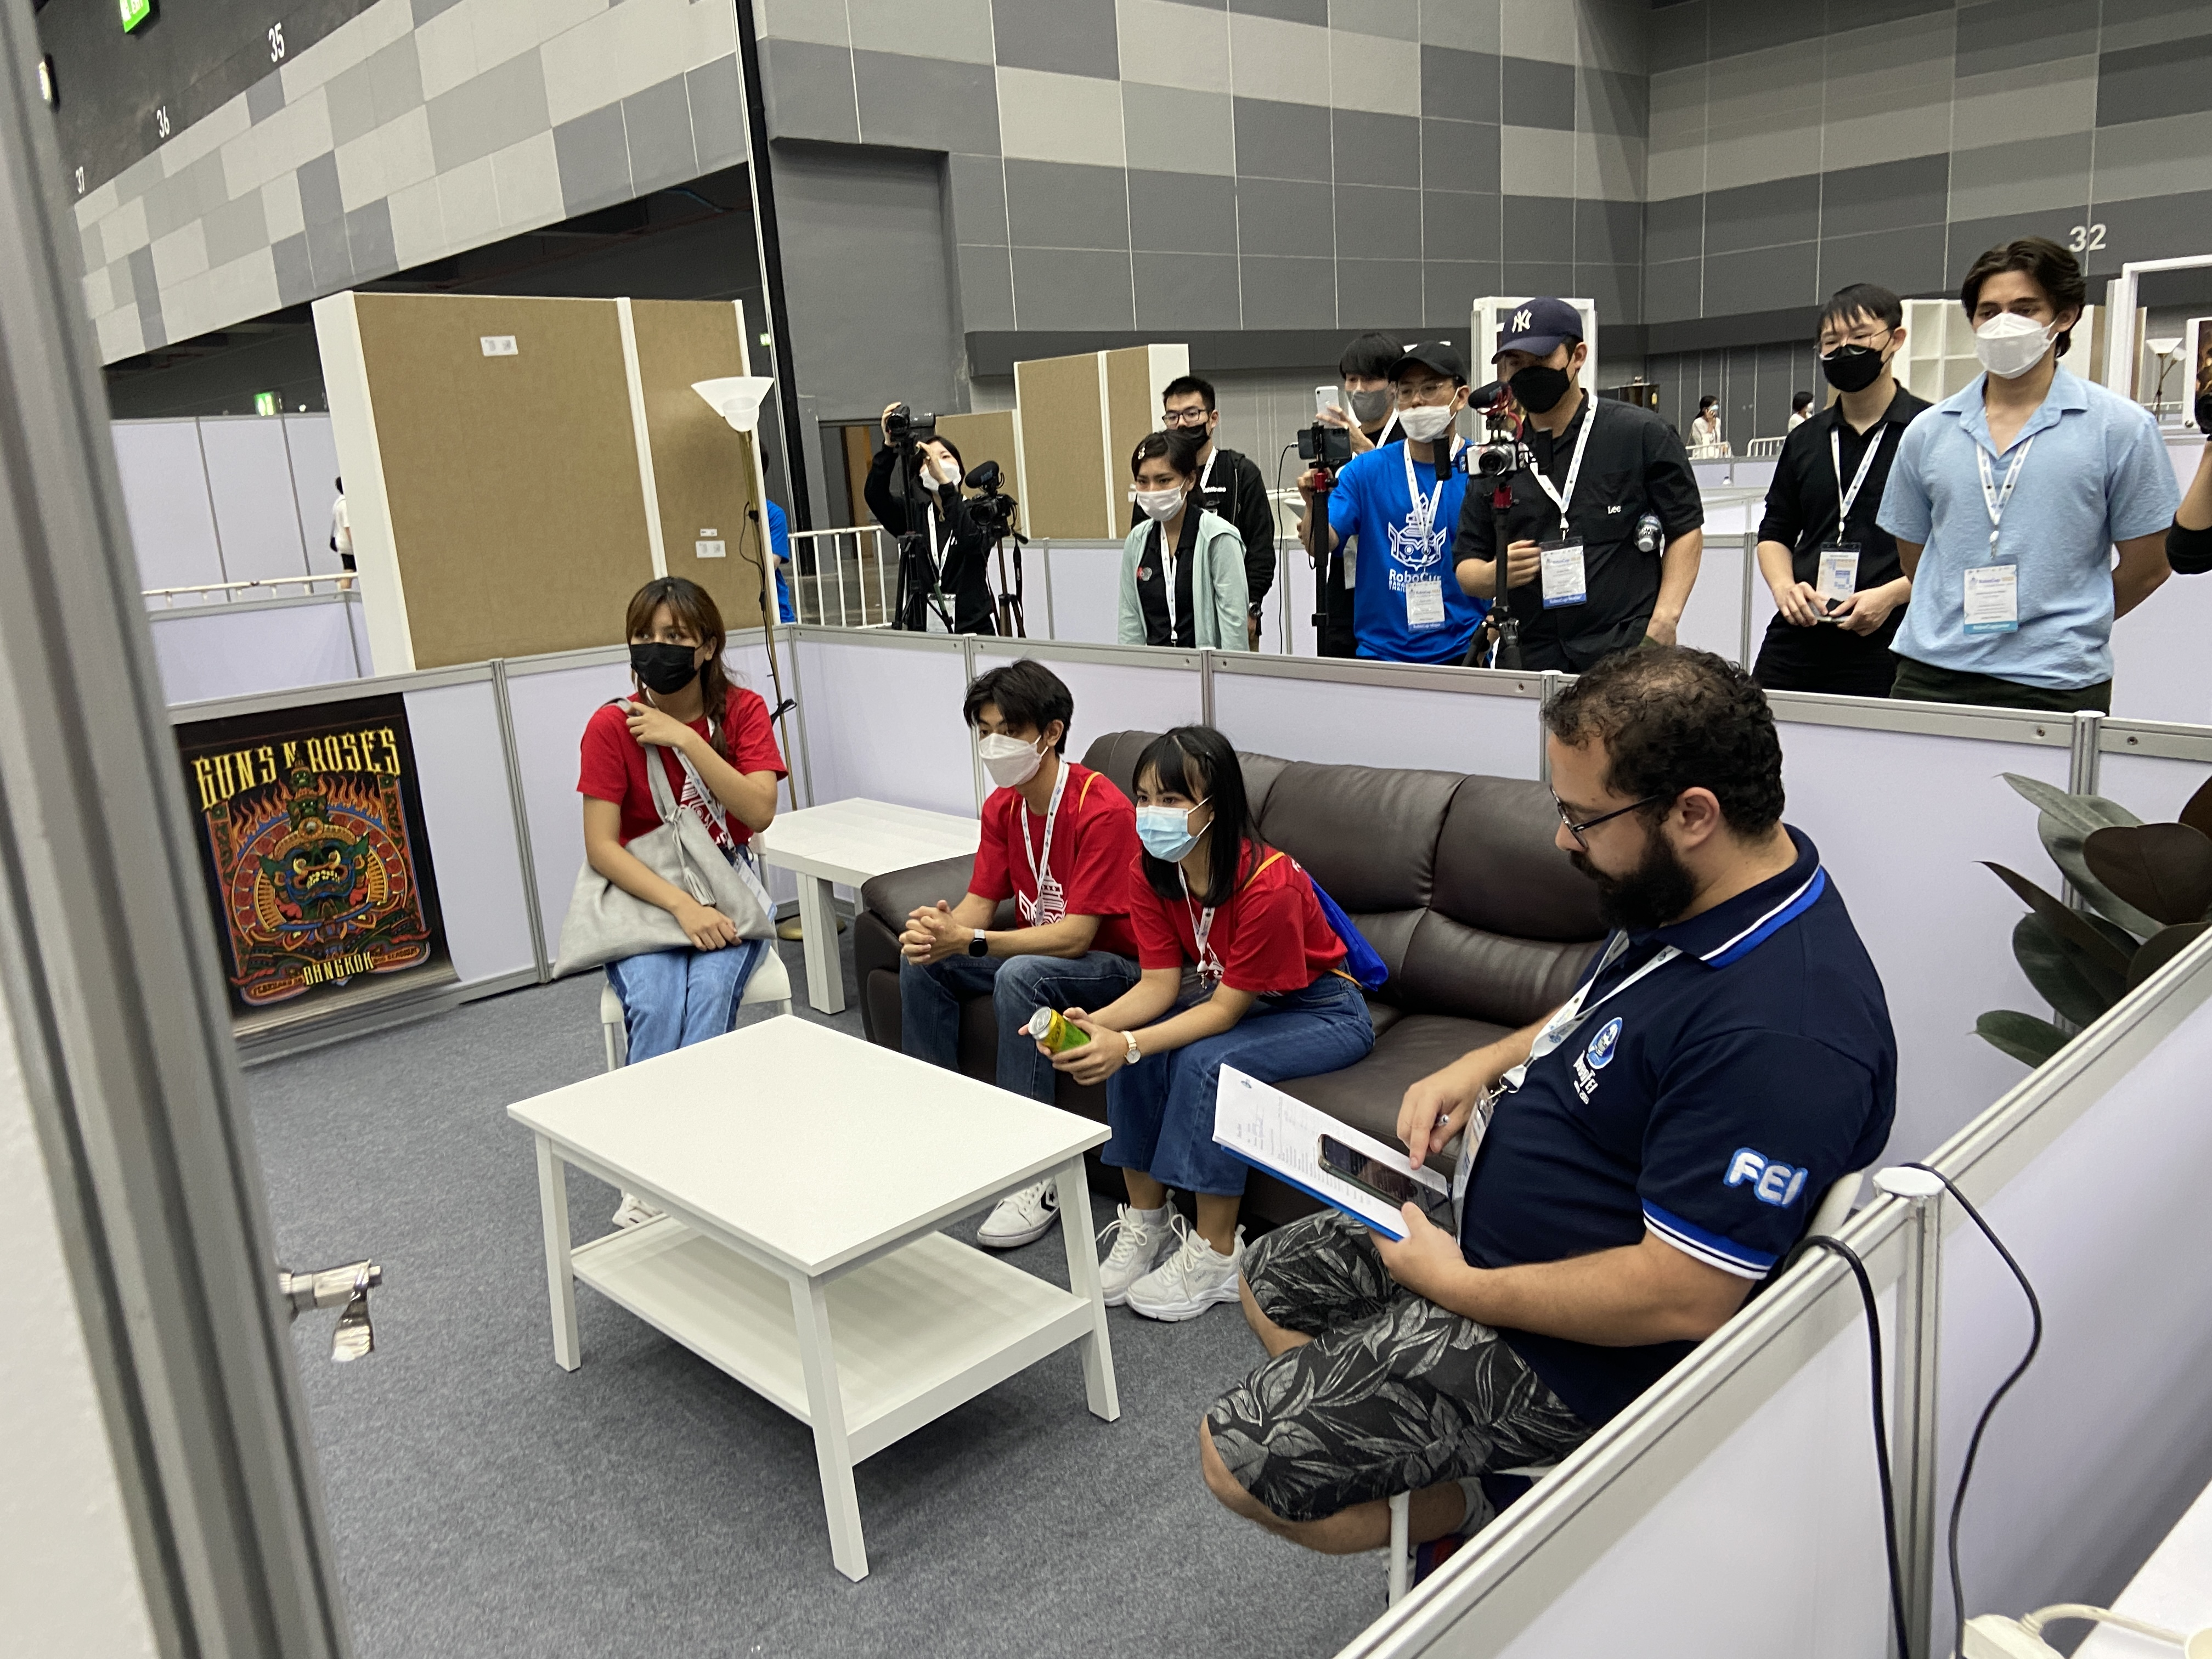
\includegraphics[height=2.2cm]{images/robocup/FMM_onsite_overview_1.jpg}
  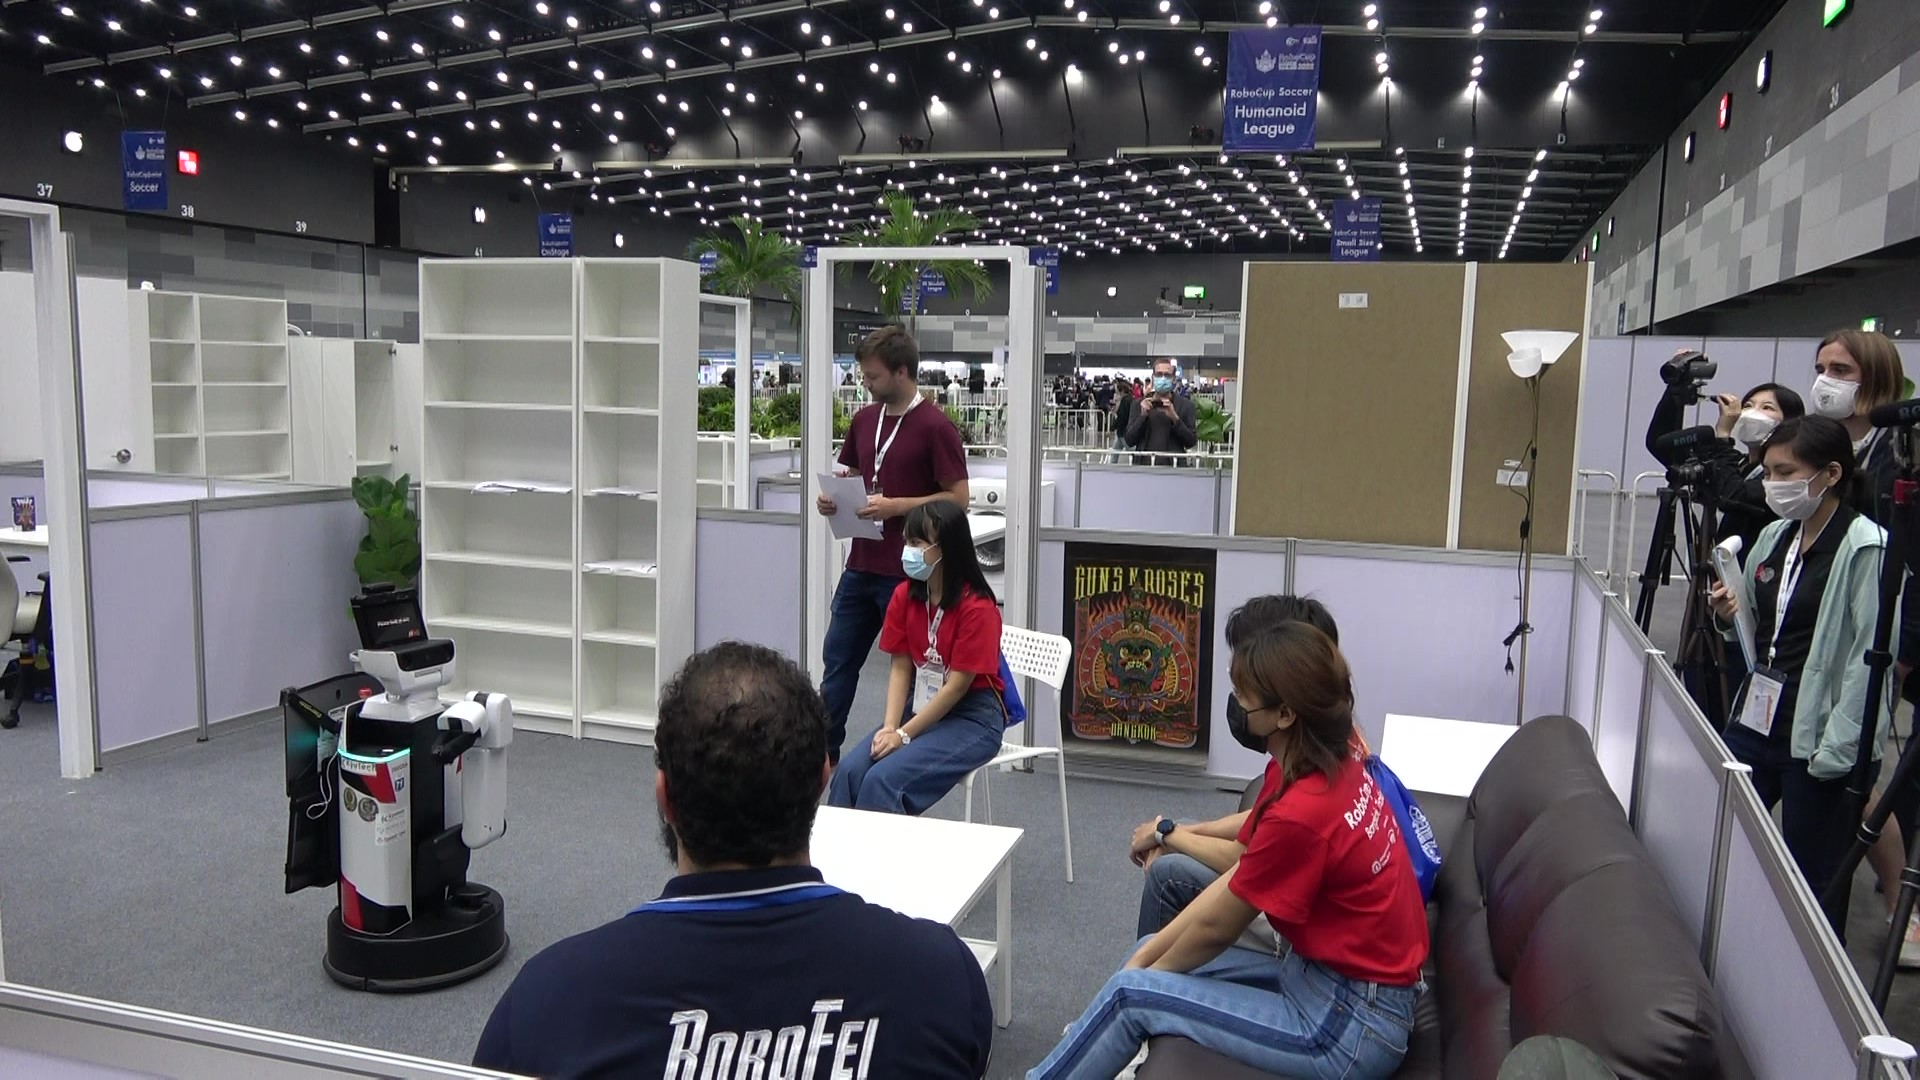
\includegraphics[height=2.2cm]{images/robocup/FMM_onsite_overview_3.jpg}
  \caption{FMMが行われた実際の会場}
  \label{onsite_overview_1}
\end{figure}


\section{現地実験}
\subsection{実験概要}
RoboCup@HomeのDSPLでは,HSRにPCを接続して使用することが認められている.
本研究で使用したPC環境は,CPU:Intel core, GPU:Geforce RTX 1080,メモリ:64GB,OS:Ubuntu18.04である.

\subsection{実験結果}
1度目のトライでは,ナビゲーションの目的地がゲストから遠い位置であったため,
遠距離から認識することとなり,不鮮明・不明瞭な画像を取得することとなった.
人物検出と3次元の位置推定は正常に動作したが,画像が不鮮明であったため,属性推定に失敗した.
また,音声認識では認識結果を得ることが出来ず,QRコードによるバイパスを用いた.
結果は,属性推定の結果があっていないこと,ヘッドディスプレイに表示した人物画像が不明瞭であったため,
0点であった.

2度目のトライは,1度目にあったナビゲーションの目的地が遠いという問題点を修正してから行った.
その結果,人物をより近い位置から認識することが出来たため,
鮮明な画像を得ることができ,属性推定も間違いなく動作した.
しかし,音声認識部においてはゲストの前までナビゲーションを行うことは出来ていたが,
名前を聞き取ることは出来ずまたQRコードのバイパスを使用することとなった.
2度目のトライにおいて,フィールド内の状況を説明するために生成した画像を図\ref{result_FMM_2}に示す.
\begin{figure}[ht]
  \centering
  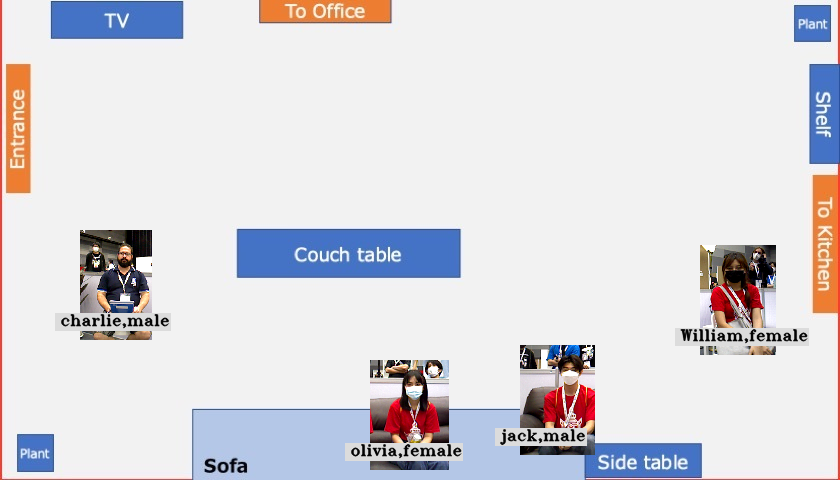
\includegraphics[width=7cm]{images/FMM/mapimage.png}
  \caption{2回目のトライで作成したマップイメージ}
  \label{result_FMM_2}
\end{figure}

% 参加チームごとのFMMで取得した点数を表\ref{fmm_points_eachcheam}にまとめる.
% \begin{table}[h]
% \begin{tabular}{ll}
%                              & Find My Mates \\
% Hibikino-Musashi@Home (ours) & \textbf{1000} \\
% Tech United Eindhoven        & \textbf{1000} \\
% Team ORIon                   & 0
% \end{tabular}
% \label{fmm_points_eachcheam}
% \end{table}


\section{考察}

\subsection{音声認識について}
今回の現地実験では,FMMを2回実施したが,いずれも音声認識の結果を得ることは出来なかった.
% 原因として,音声認識中のGraphical User Interface(GUI)が発話者に伝わっておらず,音声認識時間外に発話されたことと,発話者の声量が小さく認識が困難であったことが考えられる.
1つ目の原因として,音声認識時間外に発話されたことが挙げられる.
まず,HSRはマイクとスピーカが別デバイスであるため,HSRが発話している間に音声認識を行うと,HSRの音声も認識してしまう恐れがある.
また,音声認識は発話の有無にかかわらず一定時間のみ行うため,発話のタイミングが音声認識の結果に大きく影響してしまう.
そこで,HSRのヘッドディスプレイに認識中を示すようなGUIを作成していたが,このGUIが発話者に伝わっておらず認識時間外に発話されることがあった.
2つ目の原因として,発話者の近くまでナビゲーション出来なかったことが挙げられる.
バンコクで実際に使用された会場では,ゲストの座っているソファの手前にテーブルがあったため,ゲストの手前まで移動することが出来なかった.
そのため,遠い位置からの認識となり,発話者の音声が非常に小さくなってしまった.
このことから,音声認識の結果を得ることが困難であったと考えられる.
今後は,発話のタイミングに応じて音声認識を開始,終了するような機能を作成する必要があると考える.
また,発話者の音声が小さいことも考慮して,音声強調\cite{voice_enhancement_1, voice_enhancement_2}の技術を活用する必要があると考える.


\section{結論}
本研究では,国際的な競技会であるRoboCup@Homeで行われるFMMに向けての解法を提案し,実機実装を通してその性能評価を行った.
現地実験で,2回目のトライで満点を取得し,提案手法の有効性を示した.
一方で,音声認識やナビゲーションに関しての課題点も見つかったため,今後はこれらの課題を解決するために研究を続けていく必要がある.

\begin{thebibliography}{99}
%\small

\bibitem{robocup_hp}
RoboCup@Home. https://www.robocup.org/domains/3, (Accessed 2022-09-01).

\bibitem{hsr_paper}
% T. Yamamoto, K. Terada, A. Ochiai, F. Saito, Y. Asahara, and K. Murase, Development of Human Support Robot as the research platform of a domestic mobile manipulator, ROBOMECH Journal, Vol. 6, Art. no. 4, 2019.
Yamamoto, T., Terada, K., Ochiai, A., Saito, F., Asahara, Y., and Murase, K. “Development of Human Support Robot as the research platform of a domestic mobile manipulator,” ROBOMECH Journal, Vol. 6, Art. no. 4, (2019).

\bibitem{vosk}
Author, A., Author, B.:
JSAI SIGs Conference Paper Format Sample,
{\it International Journal of Examples}, Vol.~19, No.~4, pp.~1--2 (2007)

\bibitem{yolo}
第一著者, 第二著者:
人工知能学会研究会原稿フォーマットサンプル,
{\it International Journal of Examples}, Vol.~19, No.~4, pp.~1--2 (2007)

\bibitem{vosk_hp}
https://alphacephei.com/vosk/


\bibitem{sainburg2020finding}
Sainburg, T., Thielk, M., and Gentner, T. Q.,
% Sainburg, Tim and Thielk, Marvin and Gentner, Timothy Q
“Finding, visualizing, and quantifying latent structure across diverse animal vocal repertoires,”
{\it Public Library of Science PLoS computational biology},
Vol.16,
No.10,
pp.e1008228,
2020.

\bibitem{light-openpose}
Osokin, D. "Real-time 2d multi-person pose estimation on cpu: Lightweight openpose." arXiv preprint arXiv:1811.12004 (2018).
% Osokin, Daniil. "Real-time 2d multi-person pose estimation on cpu: Lightweight openpose." arXiv preprint arXiv:1811.12004 (2018).

\bibitem{voice_enhancement_1}
  % author = {Serrà, Joan and Pascual, Santiago and Pons, Jordi and Araz, R. Oguz and Scaini, Davide},
Serrà, J. and Pascual, S. and Pons, J. and Araz, R. O. and Scaini, D. “Universal Speech Enhancement with Score-based Diffusion,” arXiv (2022).

\bibitem{voice_enhancement_2}
% Simon Welker, Julius Richter and Timo Gerkmann. "Speech Enhancement with Score-Based Generative Models in the Complex STFT Domain", ISCA Interspeech, 2022.
Welker, S., Richter, J., and Gerkmann, T. "Speech Enhancement with Score-Based Generative Models in the Complex STFT Domain", ISCA Interspeech, (2022).

\end{thebibliography}

\end{document}
